
\begin{frame}{Overview}
  Our UI2I transformation consists of:
  \begin{enumerate}
    \item A deep UI2I estimator (GAN).
    \item A physical estimator calibrated to perform thermal UI2I.
    \item Fusion of deep and physical estimators (PETIT-GAN).
  \end{enumerate}
\end{frame}

\subsection{Deep Estimator}
\begin{frame}{Models}
  \begin{itemize}
    \item Generative Adversarial Networks(GANs):
    \begin{enumerate}
      \item CycleGAN \cite{CycleGAN2017} (cycle consistency).
      \item Contrastive Unpaired Translation (CUT) \cite{park2020cut} (contrastive learning).
    \end{enumerate}
    \item Both models share the same generator implementation.
  \end{itemize}
  \begin{figure}
    \centering
    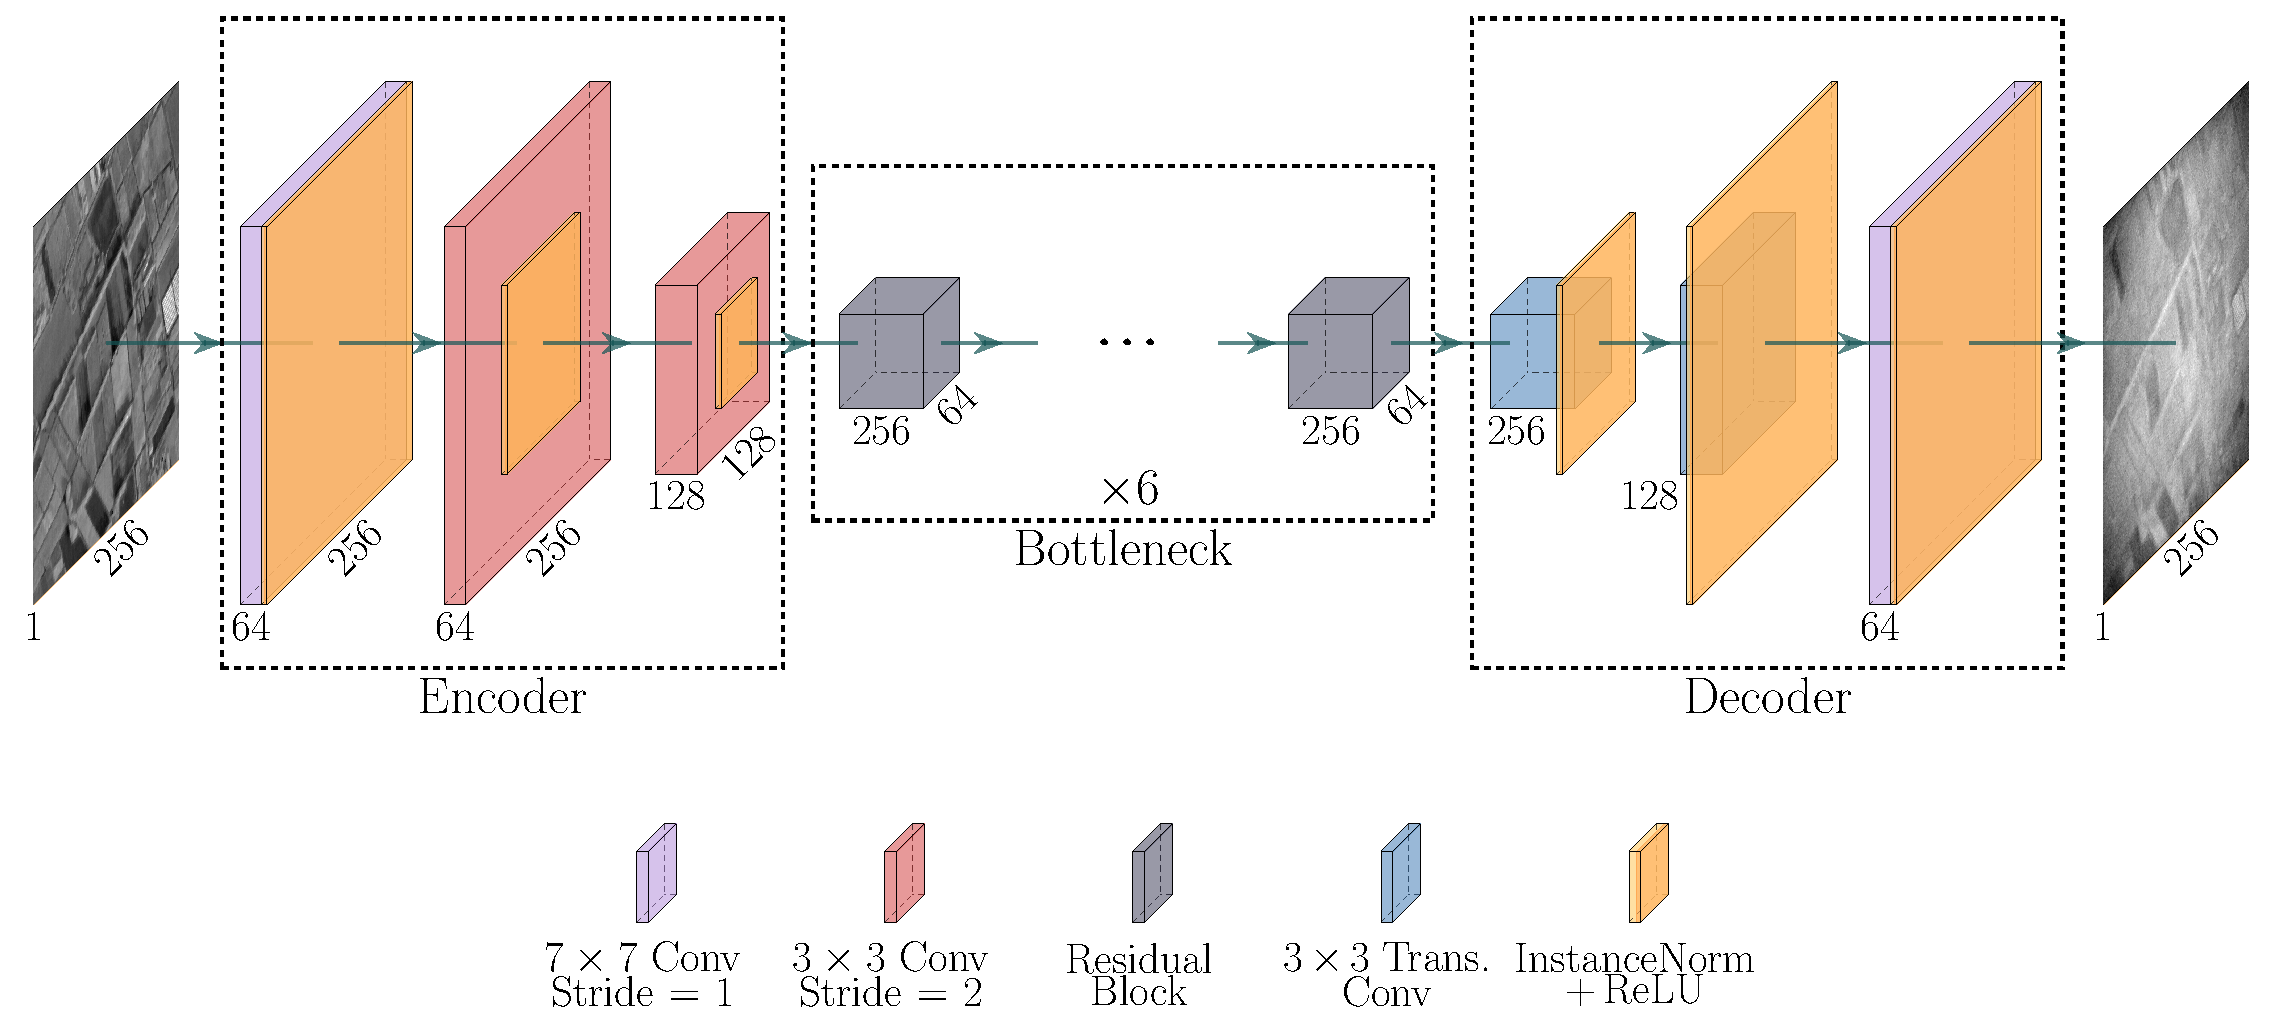
\includegraphics[width=0.7\linewidth]{../figs/network/src/cut.pdf}
  \end{figure}
\end{frame}

\subsection{Physical Estimator}

\begin{frame}{Thermal Imaging}
  \begin{itemize}
    \begin{exampleblock}{Stephan-Boltzmann}
      \begin{equation*} \label{eq:stephan-boltzmann-ideal}
        I(T_\mathit{obj}) = \int_0^\infty \frac{2\pi hc^2}{\lambda^5}\frac{1}{e^{\frac{hc}{\lambda kT_\mathit{obj}}} - 1} d\lambda = \frac{\sigma}{\pi} T_\mathit{obj}^4 \; \; \left[W sr^{-1} m^{-2}\right]
      \end{equation*}
    \end{exampleblock}  
    \item Nugent et al. \cite{10.1117/1.OE.52.6.061304}: dependency on the camera's intrinsic temperature ($T_\mathit{int}$) through 3rd order polynomials:
    \begin{equation*} \label{eq:IntensityVsTemperatures}
      \begin{split}            
        I(T_\mathit{obj}, T_\mathit{int}) &= p^{(0)}_c(T_\mathit{int}) T^4_\mathit{obj} + p^{(1)}_c(T_\mathit{int})\\
        p^{(i)}_c(T_\mathit{int}) &= \sum_{k=0}^3  c_{i,k} T_\mathit{int}^k
    \end{split}
    \end{equation*}
  \end{itemize}
\end{frame}

\begin{frame}{Physical UI2I (Our Contribution)}
  \begin{columns}   
    \begin{column}{0.5\textwidth}
      \begin{itemize} 
        \item Calibrate 2 thermal transformations:
        \begin{enumerate}
          \item $I_\mathit{pan}, T_\mathit{pan} \Rightarrow \hat{T}_\mathit{obj}$ \vspace{0.15cm}
          % \begin{equation*}
          %   \hat{T}_\mathit{obj} = \sqrt[\leftroot{5} 4]{\frac{\pmb{I_\mathit{pan}} - p^{(0)}_{c_\mathit{pan}}(\pmb{T_\mathit{pan}})}{p^{(1)}_{c_\mathit{pan}}(\pmb{T_\mathit{pan}})}}
          % \end{equation*}
          \item $\hat{T}_\mathit{obj}, T_\mathit{mono} \Rightarrow \hat{I}_\mathit{mono}$\vspace{0.25cm}
          % \begin{equation*}
          %   \hat{I}_\mathit{mono} = p^{(1)}_{c_\mathit{mono}}(\pmb{T_\mathit{mono}}) \pmb{\hat{T}_\mathit{obj}}^4 + p^{(0)}_{c_\mathit{mono}}(\pmb{T_\mathit{mono}})
          % \end{equation*}
        \end{enumerate}
        \item Cascade the transformations to get a complete panchromatic to monochromatic UI2I model: 
        \begin{equation*}
          I_\mathit{pan} \Rightarrow \hat{I}_\mathit{mono} 
        \end{equation*}
      \end{itemize}
    \end{column} 
    \begin{column}{0.5\textwidth}
      \begin{figure}            
        \centering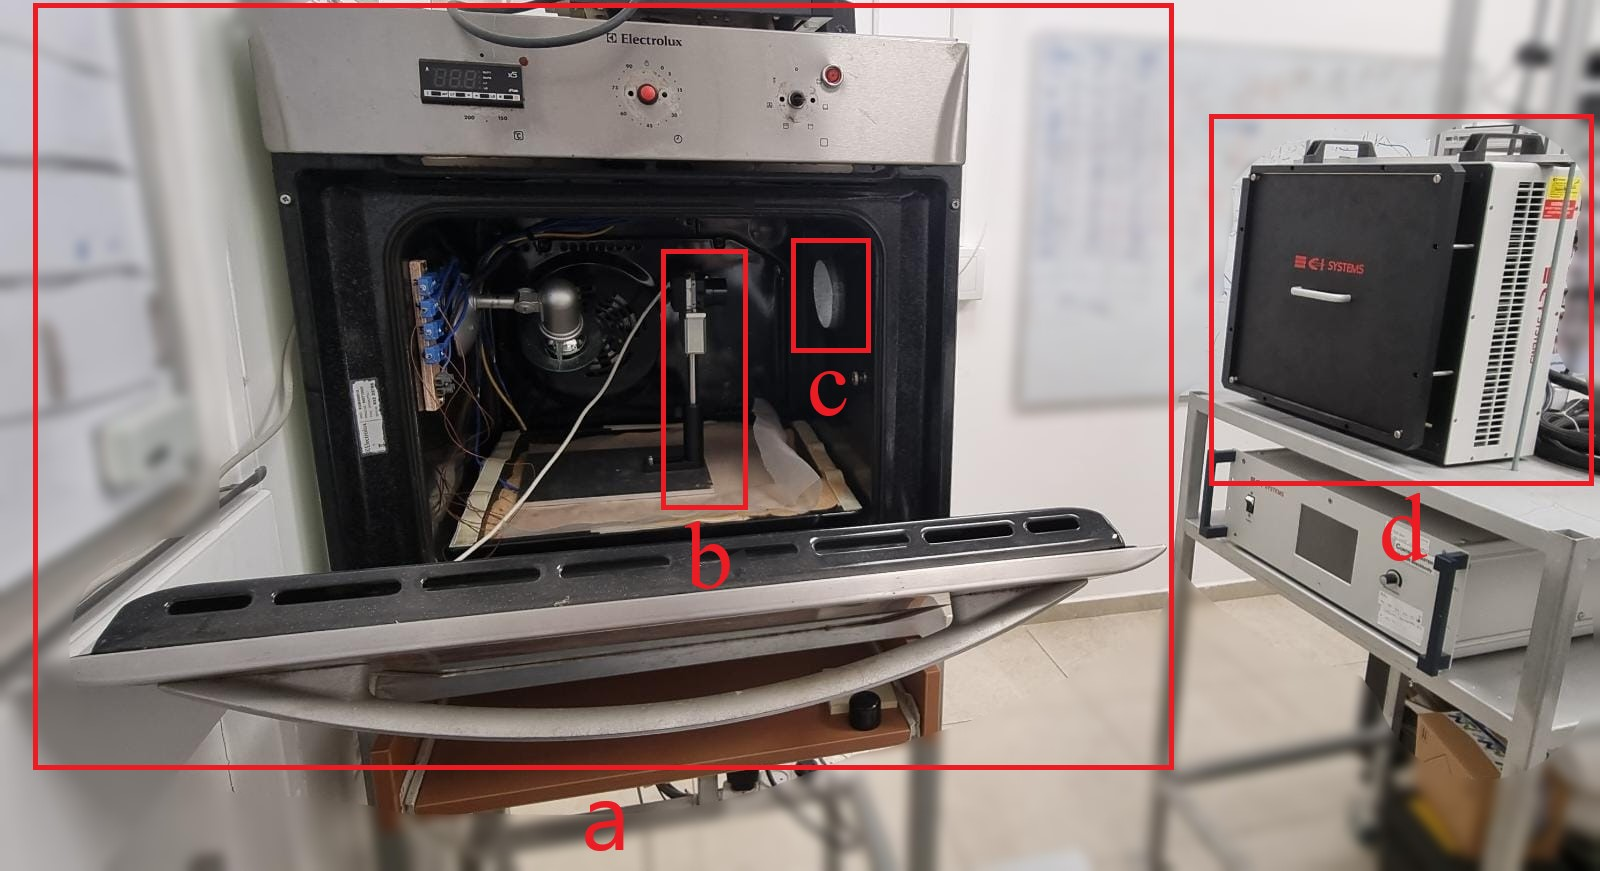
\includegraphics[width=0.75\textwidth]{../figs/methods/calib_setup.jpg}
        \caption*{Calibration Setup}
      \end{figure}      
      
    \end{column} 
  \end{columns}
\end{frame}

\subsection{PETIT}
\begin{frame}{Fusion of Estimators}
  \begin{figure}
    \centering
    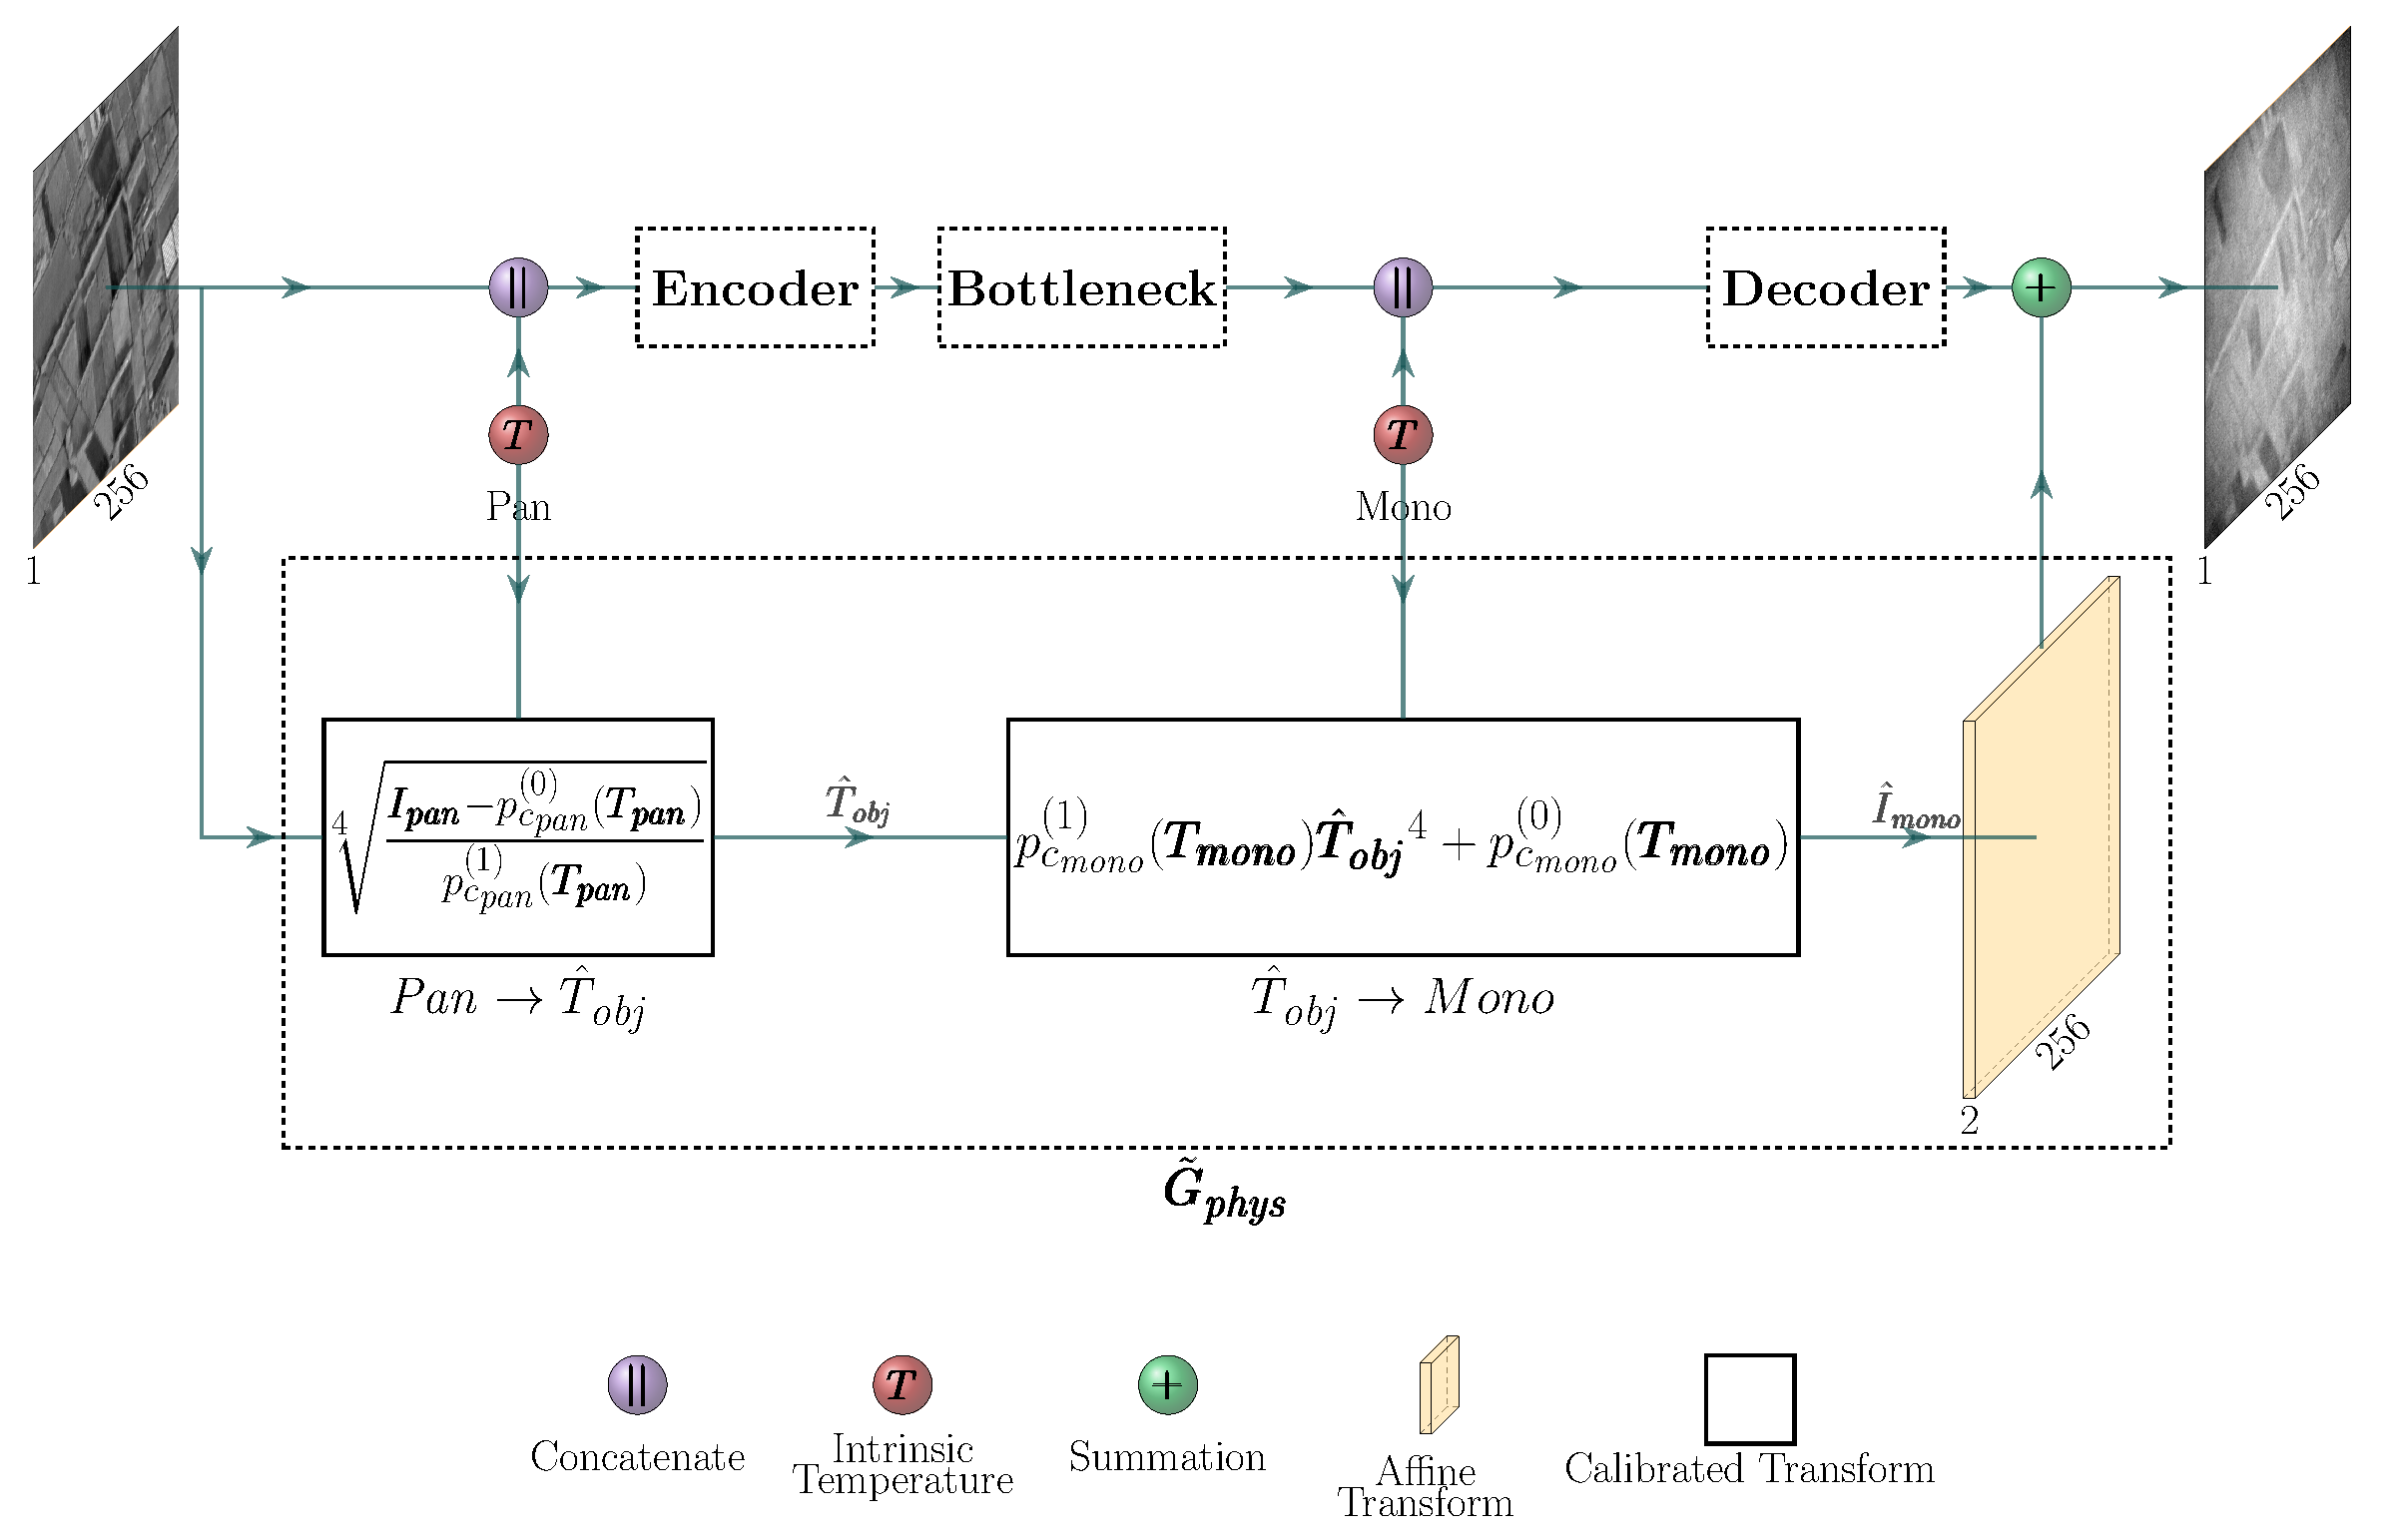
\includegraphics[width=0.65\linewidth]{../figs/network/src/petit.pdf}
  \end{figure}
\end{frame}
